\documentclass[10pt,aspectratio=169]{beamer}
\graphicspath{{./figures/}{./logos/}}
\usetheme[progressbar=frametitle, sectionpage=none]{metropolis}
\usepackage{appendixnumberbeamer}
\usepackage{siunitx}
\usepackage{framed}
\usepackage{color}
\usepackage{hyperref}
\hypersetup{
colorlinks, urlcolor=blue, linkcolor={blue!10!black},
%citecolor={blue!50!black}
}
%
% metropolis theme: https://github.com/matze/mtheme
%
\mode<presentation>
{
  \usetheme{metropolis}      % or try Darmstadt, Madrid, Warsaw, ...
  %\usecolortheme{default} % or try albatross, beaver, crane, ...
  %\usefonttheme{default}  % or try serif, structurebold, ...
  \setbeamertemplate{navigation symbols}{}
  \setbeamertemplate{caption}[numbered]
} 
\definecolor{kitwaregray}{HTML}{686868}
\definecolor{kitwarelightgray}{HTML}{EEEEEE}
\definecolor{kitwareblue}{HTML}{005F9E}
\definecolor{kitwaregreen}{HTML}{009D49}
\definecolor{kitwarewhite}{HTML}{FFFFFF}
\definecolor{kitwareblack}{HTML}{000000}
\definecolor{shadecolor}{HTML}{EEEEEE}

\setbeamercolor{progress bar}{fg=kitwaregreen}
% Theme colors are derived from these two elements
%\setbeamercolor{alerted text}{fg=}
\setbeamercolor{frametitle}{bg=kitwareblue}
\setbeamercolor{footline}{bg=kitwaregreen}
\setbeamerfont{frame numbering}{size=\small}
\setbeamertemplate{footline}{%
  \begin{beamercolorbox}[wd=\textwidth, sep=1ex]{footline}%
    %\usebeamerfont{page number in head/foot}%
    \usebeamertemplate*{frame footer}
    \hfill%
    \usebeamertemplate*{frame numbering}
  \end{beamercolorbox}%
}
% At the logo on top of the footline.
\addtobeamertemplate{footline}{\hfill
\includegraphics[height=0.45cm]{klogo_new_crop}\hspace*{0.5em}\par}{}
%\setbeamertemplate{frame footer}{
\includegraphics[width=.1\textwidth]{klogo_new_crop}}


\title{Methods for quantitative characterization of bone injury from computed-tomography images}
%\subtitle{Methods for quantitative characterization of bone injury from computed-tomography images}
\date{\today}
\author{Pablo Hernandez-Cerdan\textsuperscript{a}, Beatriz Paniagua\textsuperscript{a}, Jack Protero\textsuperscript{b}, J.S Marron\textsuperscript{b}, Eric Libingston\textsuperscript{c}, Ted Bateman\textsuperscript{c} and Matthew McCormick\textsuperscript{a}}
\institute{\textsuperscript{a} Kitware, Inc.\newline\textsuperscript{b} Dept. of Statistics and Operations Research, UNC\newline\textsuperscript{c} Dept. of Biomedical Engineering, UNC}

\titlegraphic{
\begin{tikzpicture}[overlay, remember picture]
\node[at=(current page.south), anchor=south] {%

\includegraphics[width=.3\textwidth]{klogo}\hspace{2cm} 
\includegraphics[width=.3\textwidth]{unclogo}
};
\end{tikzpicture}
}
% \titlegraphic{\hfill\includegraphics[height=1.5cm]{logo.pdf}}

\begin{document}

\maketitle

% \begin{frame}{Table of contents}
%   \setbeamertemplate{section in toc}[sections numbered]
%   \tableofcontents[hideallsubsections]
% \end{frame}

\section{Introduction}

\begin{frame}[fragile]{Introduction}
\begin{itemize} \itemsep1em
\item Bone diseases are present in 50\% adults in the United States (CDC 2012)

\item Imaging provides a fast, scalable and non-invasive to examine bone structure. But the evaluation is often performed qualitatively or semi-quantitative.

\item Our goal is to present open source software tools to quantify musculoskeletal diseases through imaging.

\item These methods are tested on mouse femur wound model images obtained during a hemophilia study.
\end{itemize}
\end{frame}

\section{Materials}

\begin{frame}[fragile]{Materials}
\begin{columns}[onlytextwidth]
  \column{0.25\textwidth}
    \centering
    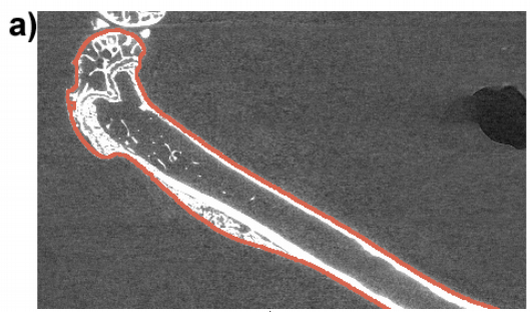
\includegraphics[width=0.99\textwidth]{figures/bone_materials_femur_highlight.png}\\
    \vspace{0.5cm}
    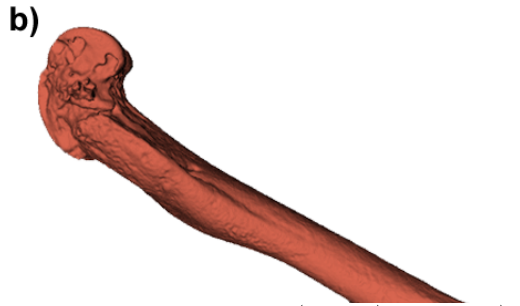
\includegraphics[width=0.99\textwidth]{figures/bone_materials_femur_3D.png}
  \column{0.75\textwidth}
    \centering
    \begin{itemize} \itemsep1em
        \item Three, 22 week old (skeletally mature), genetically modified, male mice.

        \item F8 gene knockout preventing the generation of protein coagulation factor VIII.

        \item Pathogenic pathway similar to hemophilia, presenting bleeding induced bone and joint damage.

        \item Images of right (control) and left (wounded) limbs
    \end{itemize}
\end{columns}
\end{frame}

\begin{frame}[fragile]{Materials}
\begin{itemize} \itemsep1em
\item Images acquired using microCT, with resolution of $10$\si{\micro} (\si{\micro}CT80, Scanco)
\item Trabecular bone at the proximal tibia, inferior to the growth plate
\end{itemize}
\vspace{0.5cm}
\begin{columns}[onlytextwidth]
  \column{0.5\textwidth}
    \centering
    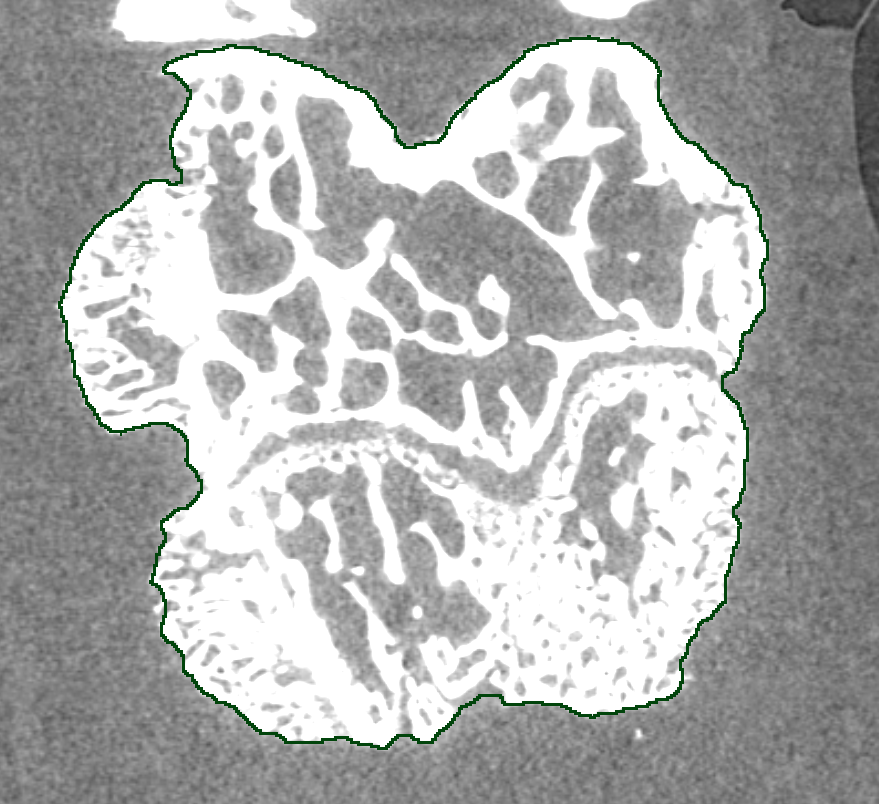
\includegraphics[width=4cm]{figures/bone_materials.png}
  \column{0.5\textwidth}
    \centering
    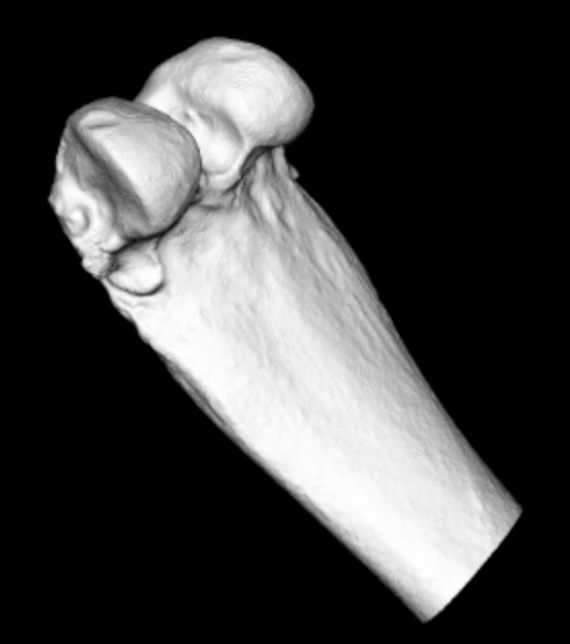
\includegraphics[width=3.7cm]{figures/bone_materials_3D.png}
\end{columns}
\end{frame}

{
\setbeamercolor{background canvas}{bg=kitwarewhite}
\begin{frame}{Image Analysis Workflow}
\begin{columns}[onlytextwidth]
    \column{0.75\textwidth}
      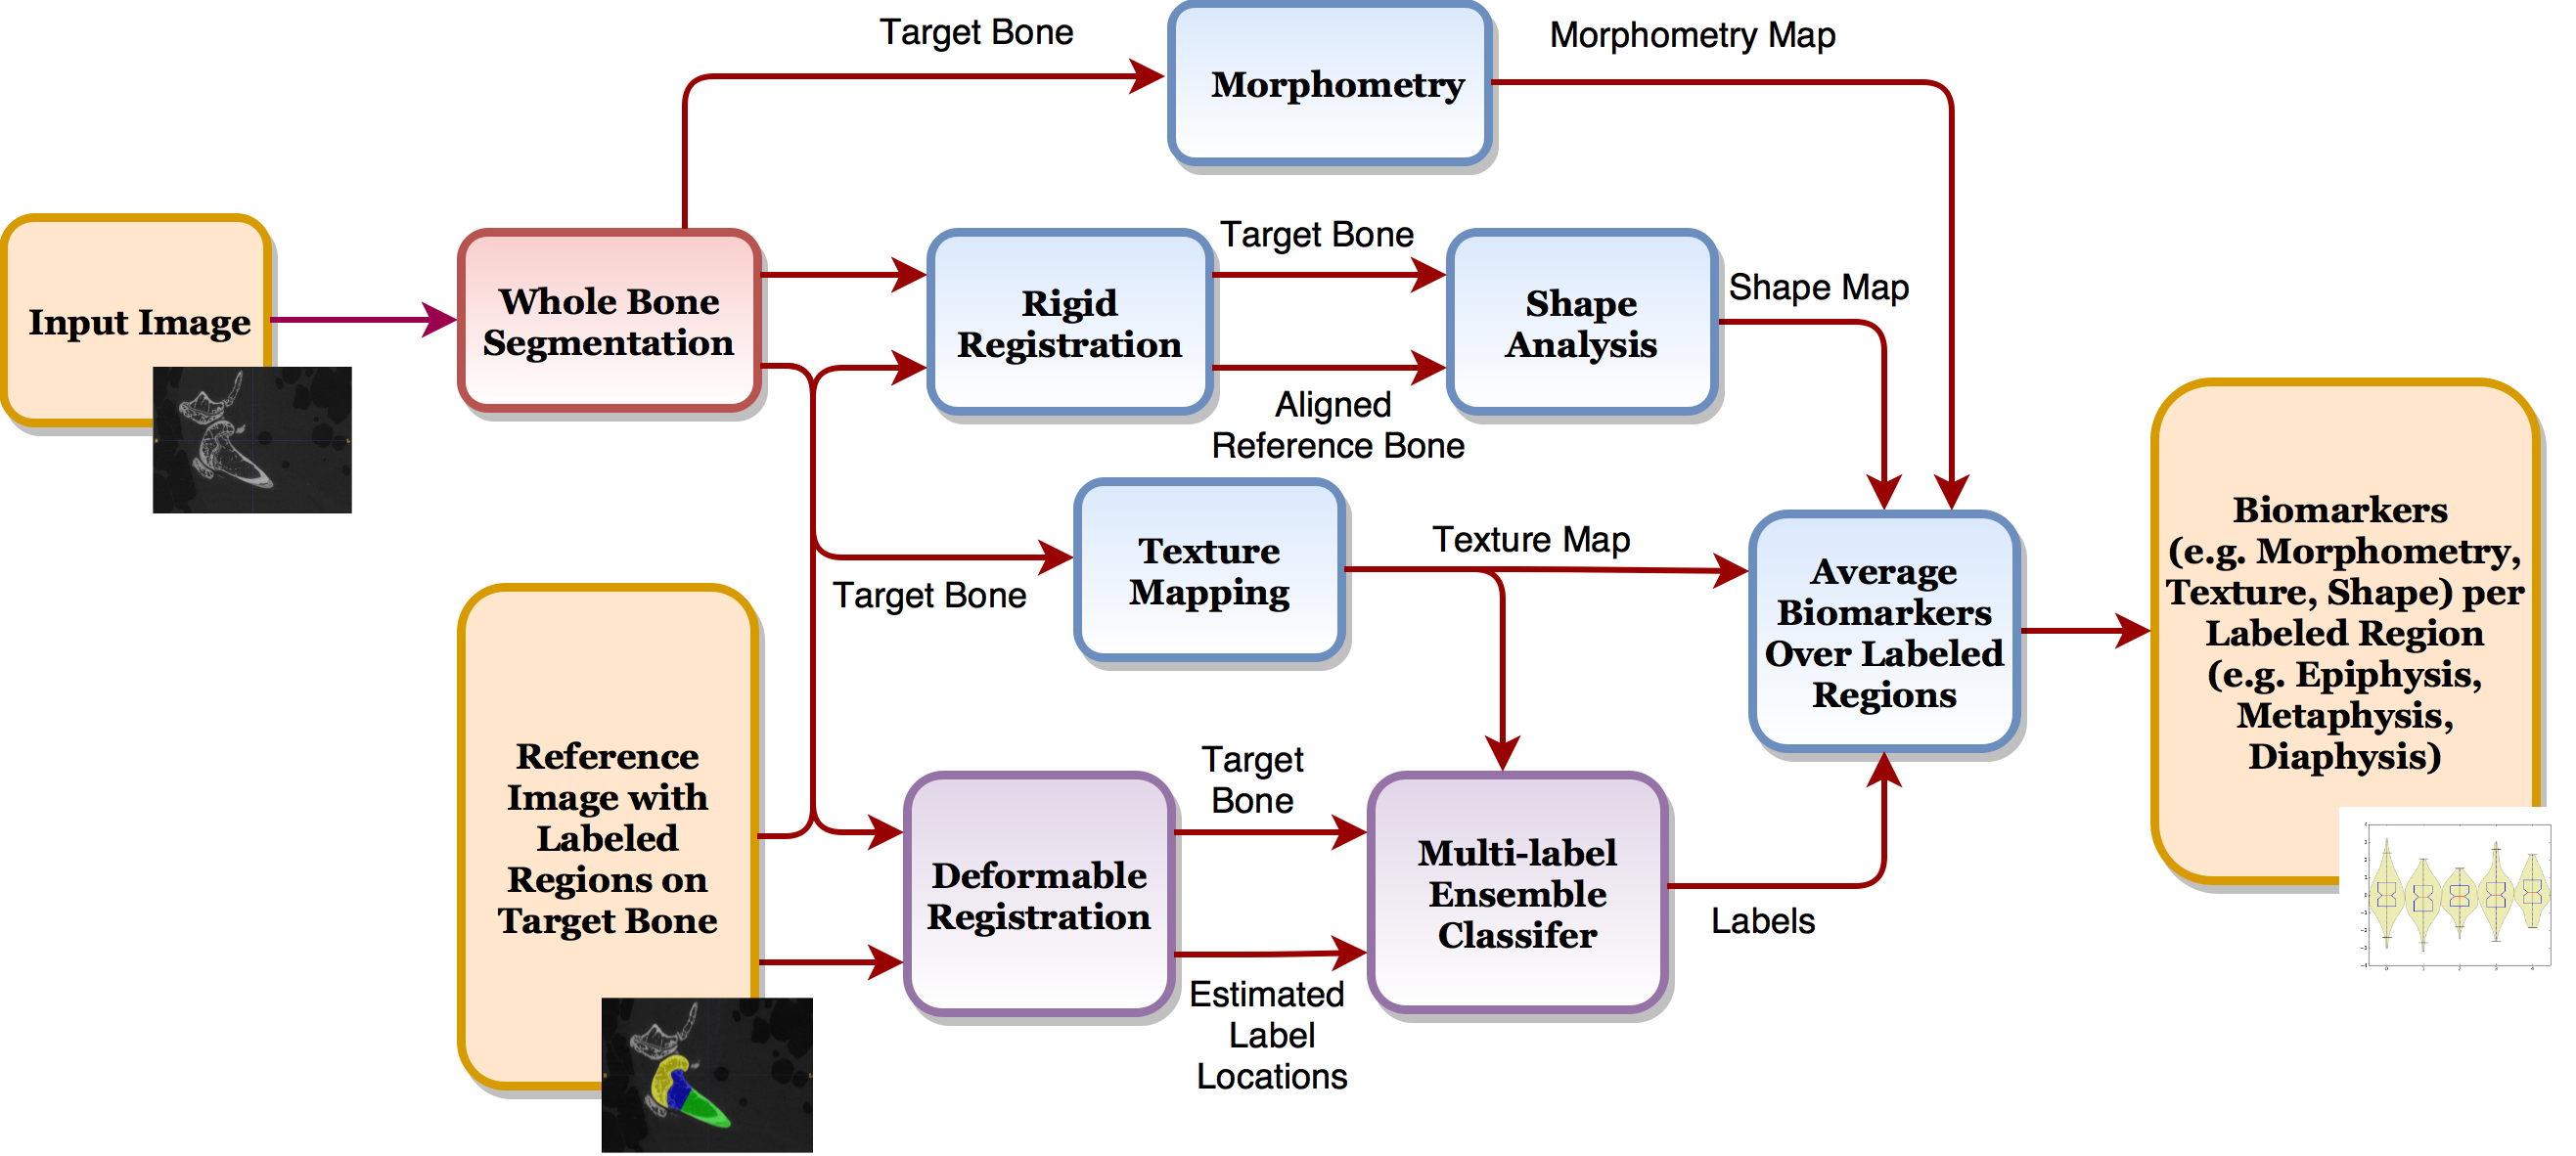
\includegraphics[width=0.99\textwidth]{figures/Automated_Processing_Pipeline.png}
        %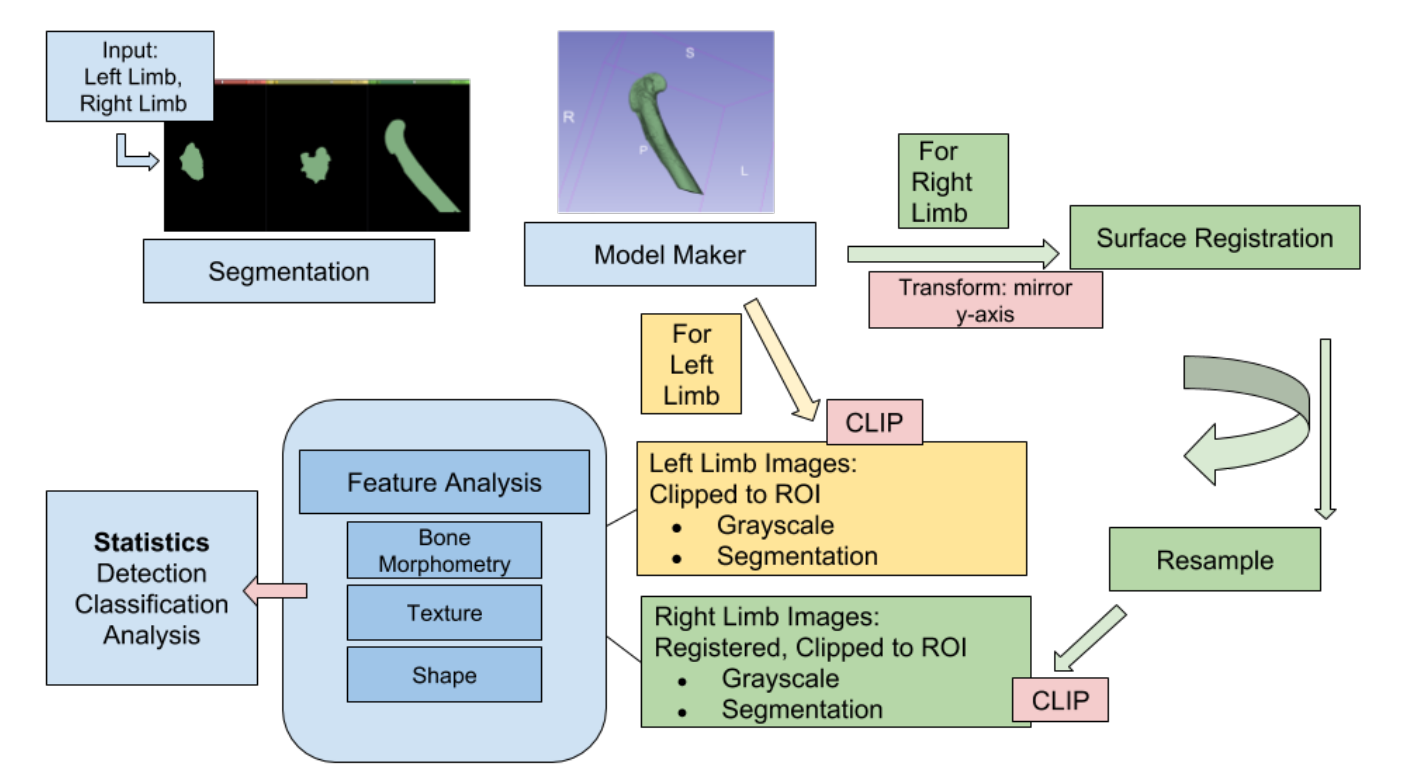
\includegraphics[width=0.99\textwidth]{figures/analysis_workflow.png}
    \column{0.25\textwidth}
        \centering
        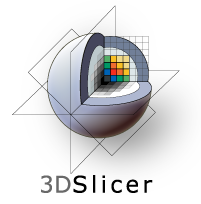
\includegraphics[width=2.5cm]{logos/logo_slicer.png}\\
        \vspace{0.3cm}
        Data and all the steps for reproducilibty at: \url{http://dx.doi.org/10.6084/m9.figshare.6947891}
\end{columns}
\end{frame}
}

\section{Methods}

\begin{frame}[fragile]{Quantitative Methods}
  \begin{itemize} \itemsep2em
    \item Texture Analysis: GLCM and GLRLM

    \item Bone Morphometry

    \item Shape Analysis: Iterative Closest Points (ICP)
  \end{itemize}
\end{frame}

\begin{frame}[fragile]{Texture Analysis}
  We investigated two different types of textural features related to different aspects of the bone architecture:
  \vspace{0.1cm}
  % \metroset{block=fill}
  \begin{exampleblock}{Co-occurrence based-features:}
    \begin{itemize} \itemsep0.8em
      \item Haralick et al. 1973 \cite{Haralick1973}
      \item Local neighborhoods and connectivities
      \item Grey Level Co-occurrence Matrix (GLCM)
    \end{itemize}
  \end{exampleblock}
  \begin{exampleblock}{Run-length based-features:}
    \begin{itemize} \itemsep0.8em
      \item Galloway et al. 1975 \cite{Galloway1975}
      \item Grey-level clusters
      \item Grey Level Run-Length Matrix (GLRLM)
    \end{itemize}
  \end{exampleblock}
\end{frame}

\begin{frame}{Texture Analysis: Co-occurrence Matrix (GLCM)}
  \begin{columns}[onlytextwidth]
    \column{0.6\textwidth}
    Eight co-occurrence based-features:
    \begin{itemize} \itemsep0.5em
      \item Energy
      \item Entropy
      \item Correlation
      \item Inverse Difference Moment (IDM)
      \item Contrast
      \item Cluster shade
      \item Cluster prominence
      \item Haralick’s correlation
    \end{itemize}
    \column{0.4\textwidth}
    \begin{columns}
    \centering
    \column{0.5\textwidth}
    \centering
    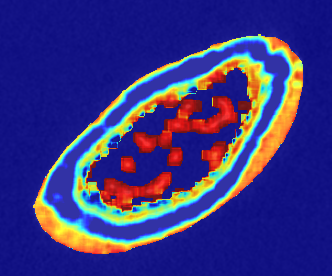
\includegraphics[width=0.9\textwidth]{./TextureMapsImages/GLRLM_49_LEFT_0_crop.png}\\
    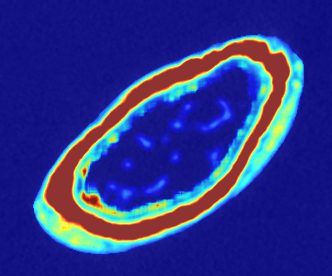
\includegraphics[width=0.9\textwidth]{./TextureMapsImages/GLRLM_49_LEFT_2_crop.png}
    \column{0.5\textwidth}
    \centering
    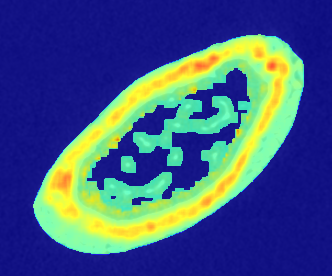
\includegraphics[width=0.9\textwidth]{./TextureMapsImages/GLRLM_49_LEFT_1_crop.png}\\
    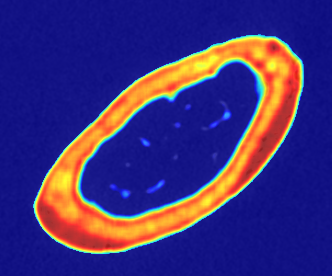
\includegraphics[width=0.9\textwidth]{./TextureMapsImages/GLRLM_49_LEFT_3_crop.png}
    \end{columns}
  \end{columns}
\end{frame}

\begin{frame}{Texture Analysis: Run-Length Matrix (GLRLM)}
  \begin{columns}[onlytextwidth]
    \column{0.6\textwidth}
    Ten run-length based-features:
    \begin{itemize}
       \item Short run emphasis (SRE)
       \item Long run emphasis (LRE)
       \item Grey level non-uniformity (GLN)
       \item Run length non-uniformity (RLN)
       \item Low grey level run emphasis (LGRE)
       \item High grey level run emphasis (HGRE)
       \item Short run low grey level emphasis (SRLGE)
       \item Short run high grey level emphasis (SRHGE)
       \item Long run low grey level emphasis (LRLGE)
       \item Long run high grey level emphasis (LRHGE)
    \end{itemize}
    \column{0.4\textwidth}
    \begin{columns}
    \centering
    \column{0.5\textwidth}
    \centering
    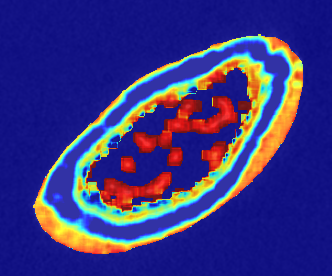
\includegraphics[width=0.9\textwidth]{./TextureMapsImages/GLRLM_49_LEFT_0_crop.png}\\
    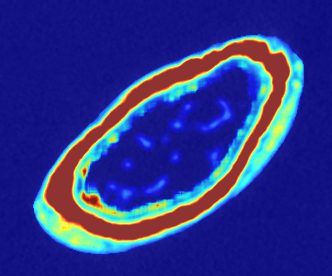
\includegraphics[width=0.9\textwidth]{./TextureMapsImages/GLRLM_49_LEFT_2_crop.png}
    \column{0.5\textwidth}
    \centering
    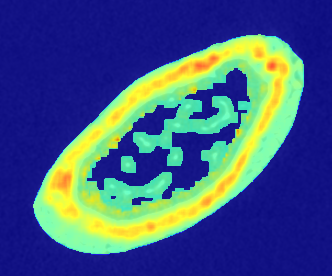
\includegraphics[width=0.9\textwidth]{./TextureMapsImages/GLRLM_49_LEFT_1_crop.png}\\
    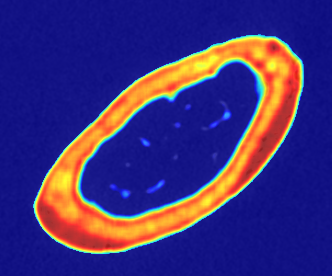
\includegraphics[width=0.9\textwidth]{./TextureMapsImages/GLRLM_49_LEFT_3_crop.png}
    \end{columns}
  \end{columns}
\end{frame}

\begin{frame}{Bone Morphometry}

  \begin{columns}[onlytextwidth]
    \column{0.6\textwidth}
    Bone morphometry features describe the 3D shape of subchondral bone trabecular structure
    Five bone morphometry features:
    \begin{itemize} \itemsep0.5em
      \item Bone volume density (Bv/Tv)
      \item Bone surface density (Bs/Bv)
      \item Trabecular thickness (Tb.Th)
      \item Trabecular separation (Tb.Sp)
      \item Trabecular number (Tb.N)
    \end{itemize}
    \column{0.4\textwidth}
    \begin{columns}
    \centering
    \column{0.5\textwidth}
    \centering
    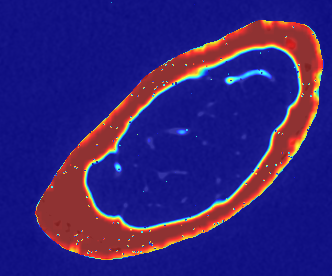
\includegraphics[width=0.9\textwidth]{./TextureMapsImages/BM_49_LEFT_0_crop.png}\\
    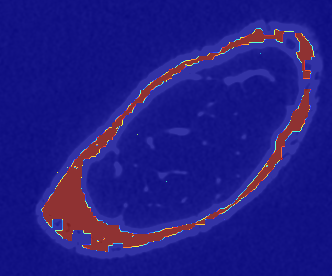
\includegraphics[width=0.9\textwidth]{./TextureMapsImages/BM_49_LEFT_2_crop.png}
    \column{0.5\textwidth}
    \centering
    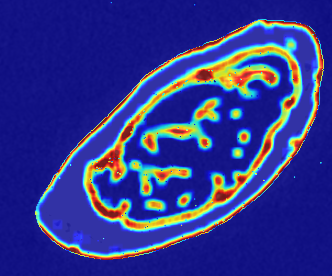
\includegraphics[width=0.9\textwidth]{./TextureMapsImages/BM_49_LEFT_1_crop.png}\\
    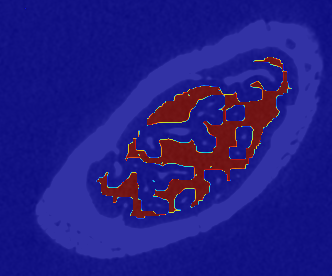
\includegraphics[width=0.9\textwidth]{./TextureMapsImages/BM_49_LEFT_3_crop.png}
    \end{columns}
  \end{columns}
\end{frame}

\begin{frame}{Shape Analysis}
  \begin{center}
  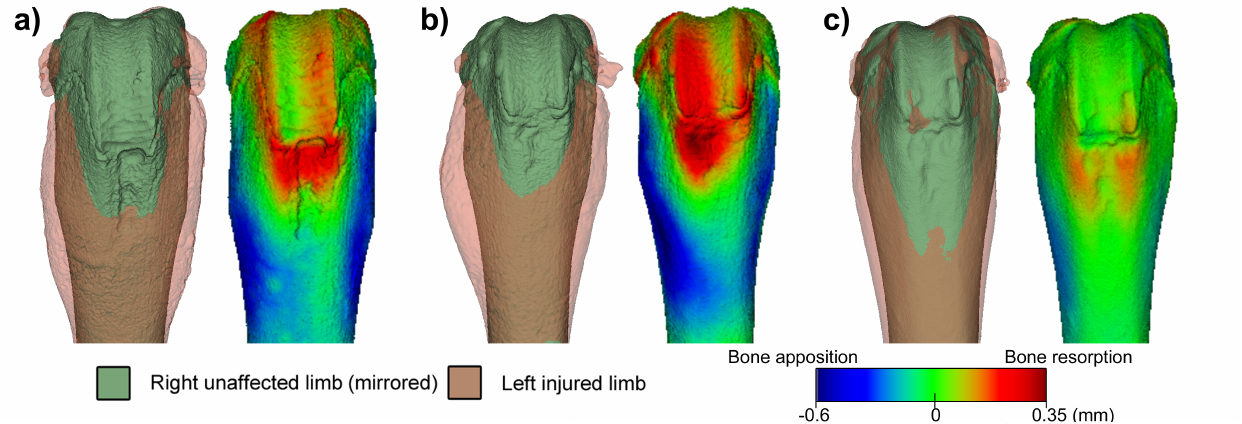
\includegraphics[width=0.9\textwidth]{./figures/analysis_shape.png}\\
  \end{center}
  \vspace{0.1cm}
  \centering
  Shape analysis results for all subjects, including superimposed 3D models (left) and visualization of pathological shape changes via signed distances (right).
\end{frame}

{
\setbeamercolor{background canvas}{bg=kitwarewhite}
\section{Results}
\begin{frame}{Results}
  \centering
  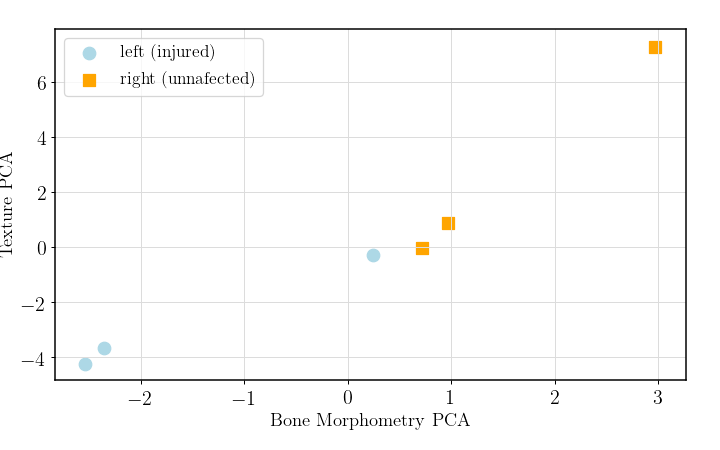
\includegraphics[width=0.7\textwidth]{./figures/features_pcaBoneVSpcaTexture1000Bins.png}\\
  \vspace{0.1cm}
  First principal component of the bone morphometry analysis versus first principal component of the texture analysis.
\end{frame}
}

\section{Conclusion}

\begin{frame}{Conclusions}
  \begin{itemize} \itemsep1.0em

    \item Computed biomarkers based on not only traditional bone morphometrics, but also texture and shape-based metrics.
  \end{itemize}

  \begin{columns}[onlytextwidth]
    \column{0.75\textwidth}
    \begin{itemize} \itemsep1.0em
      \item High performance implementation in ITK. N-dimensions. Local Texture Maps.
    \end{itemize}
    \column{0.25\textwidth}
    \centering
    
\includegraphics[width=0.8\textwidth]{./logos/logo_ITK.png}
  \end{columns}

  \begin{itemize} \itemsep1.0em
    \item Workflow can be adapted to target other modalities and pathologies.
    \item We were able to classify injured and healthy femurs with simple statistical methods.
  \end{itemize}
\end{frame}

\begin{frame}{Open Source Development}
  \begin{columns}[onlytextwidth]
    \column{0.80\textwidth}
    \metroset{block=fill}
    \begin{block}{All analysis filters were implemented as part of \textbf{ITK}, the Insight Toolkit:}
    \begin{itemize} \itemsep1.0em
      \item High performance, greatly reducing computational time in texture analysis.
      \item Able to compute 3D maps of multidimensional features
    \end{itemize}
  \end{block}
    \column{0.20\textwidth}
    \centering
    
\includegraphics[width=0.8\textwidth]{./logos/logo_ITK.png}
  \end{columns}
  \vspace{0.2cm}
  \begin{columns}[onlytextwidth]
    \column{0.80\textwidth}
    \metroset{block=fill}
    \begin{block}{\textbf{Python} packages available for Windows, Mac and Linux}
    % \noindent \textbf{Python} packages available for Windows, Mac and Linux
      \centering
      pip install itk-texturefeatures itk-bonemorphometry
  \end{block}
    \column{0.20\textwidth}
    \centering
    
\includegraphics[width=0.99\textwidth]{./logos/logo_python.png}
  \end{columns}
  \vspace{0.2cm}
  \begin{columns}[onlytextwidth]
    \column{0.80\textwidth}
    \metroset{block=fill}
    \begin{block}{Graphical interface in 3DSlicer: Bone Texture Extension}
    \end{block}
    \column{0.20\textwidth}
    \centering
    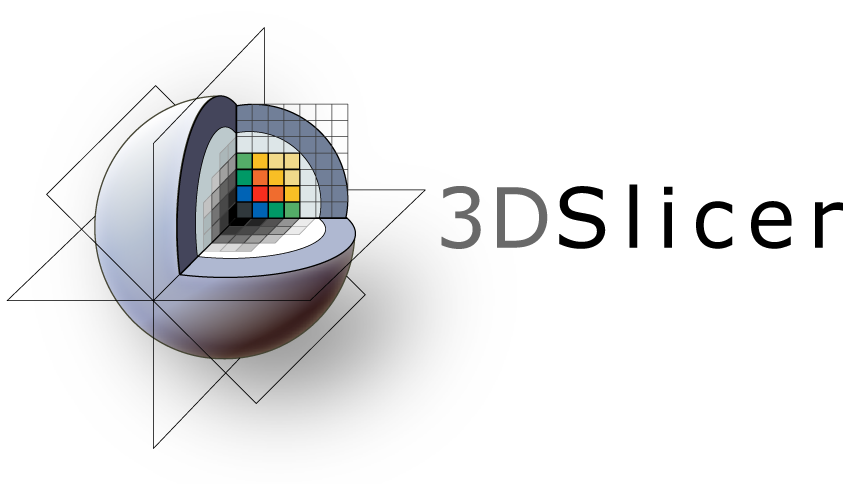
\includegraphics[width=0.9\textwidth]{./logos/logo_slicer_horizontal.png}
  \end{columns}
\end{frame}

\begin{frame}
  \begin{columns}[onlytextwidth]
  \column{0.5\textwidth}
    
\includegraphics[width=0.9\textwidth]{./logos/klogo.png}\\
    \vspace{0.1cm}
    % \metroset{block=fill}
    \begin{block}{\color{kitwareblue} Collaborative Software R\&D}
      \begin{itemize}%\itemsep0.2em
        \item Algorithms \& applications
        \item Software process \& infrastructure
        \item Support \& training
        \item Open source leadership
      \end{itemize}
    \end{block}
    \begin{block}{\color{kitwareblue} Supporting industry, goverment and academia}
    \end{block}
  \column{0.5\textwidth}
    \centering
    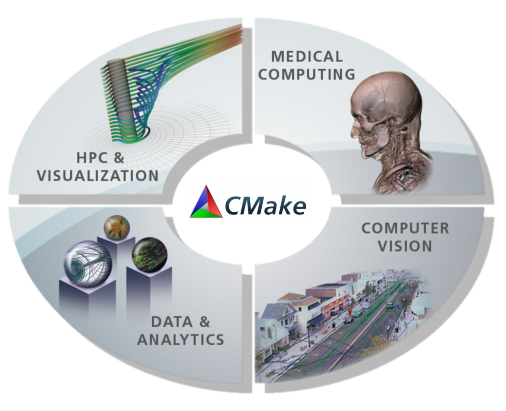
\includegraphics[width=0.9\textwidth]{./logos/kitware_pie.png}
    
\includegraphics[width=0.9\textwidth]{./logos/kitware_itk_slicer_vtk_logos.png}
  \end{columns}
\end{frame}

{
\setbeamercolor{background canvas}{bg=kitwarewhite}
\begin{frame}{Medical Computing}
    \centering
    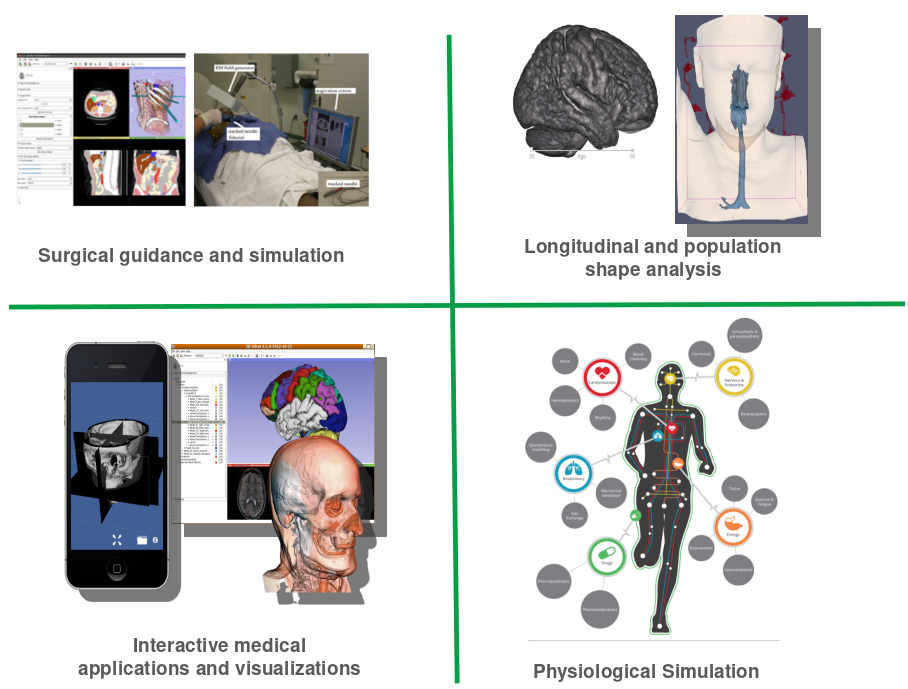
\includegraphics[height=0.9\textheight]{./logos/kitware_medical.png}
\end{frame}
}

\begin{frame}[standout]
  \centering
  {\huge Thanks!}\\
  pablo.hernandez@kitware.com\\
  \vspace{2cm}
  % {\Huge Questions?}\\
\end{frame}

\appendix

{
\setbeamercolor{background canvas}{bg=kitwarewhite}
\begin{frame}[fragile]{Performance Comparison: ITK vs Matlab (2D)}
  \centering
  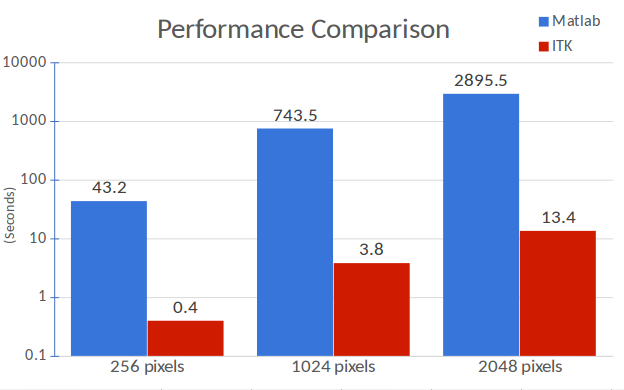
\includegraphics[height=0.9\textheight]{./figures/TextureFeaturesPerformanceComparison.png}
\end{frame}

\begin{frame}[fragile]{GLCM Matrices}
  \centering
  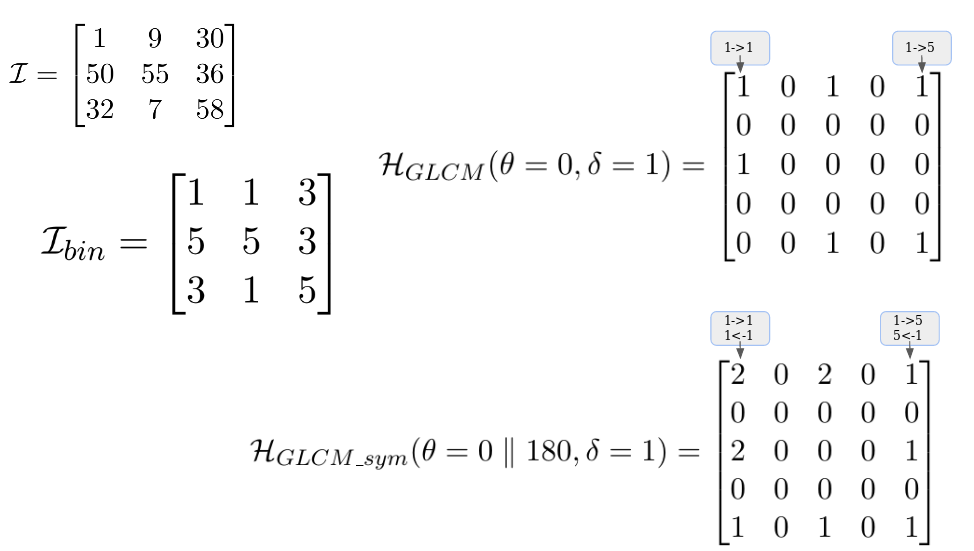
\includegraphics[width=0.9\textwidth]{./figures/GLCM_matrices.png}
\end{frame}

\begin{frame}[fragile]{GLRLM Matrices}
  \centering
  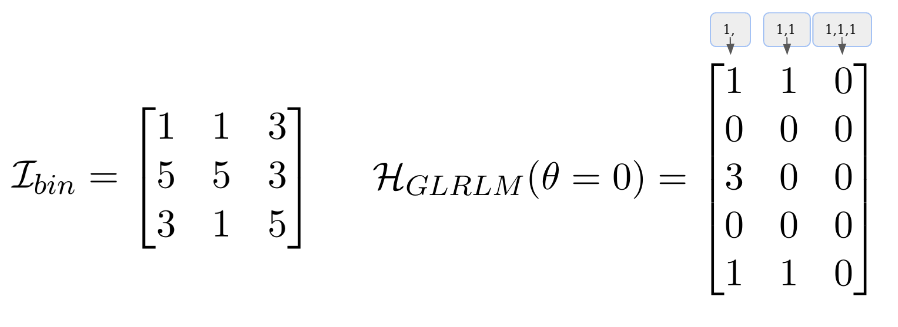
\includegraphics[width=0.9\textwidth]{./figures/GLRLM_matrices.png}
\end{frame}
}

\begin{frame}[allowframebreaks]{References}

  \bibliography{references}
  \bibliographystyle{abbrv}

\end{frame}


\end{document}

